%%
%% Beginning of file 'sample.tex'
%%
%% Modified 2005 December 5
%%
%% This is a sample manuscript marked up using the
%% AASTeX v5.x LaTeX 2e macros.

%% The first piece of markup in an AASTeX v5.x document
%% is the \documentclass command. LaTeX will ignore
%% any data that comes before this command.

%% The command below calls the preprint style
%% which will produce a one-column, single-spaced document.
%% Examples of commands for other substyles follow. Use
%% whichever is most appropriate for your purposes.
%%
%%\documentclass[12pt,preprint]{aastex}

%% manuscript produces a one-column, double-spaced document:

%\documentclass{article}
\documentclass[twocolumn]{aastex6}
%\documentclass[iop]{emulateapj}

%% preprint2 produces a double-column, single-spaced document:
%\documentclass[preprint2]{aastex}

%% Sometimes a paper's abstract is too long to fit on the
%% title page in preprint2 mode. When that is the case,
%% use the longabstract style option.

%% \documentclass[preprint2,longabstract]{aastex}

%% If you want to create your own macros, you can do so
%% using \newcommand. Your macros should appear before
%% the \begin{document} command.
%%
%% If you are submitting to a journal that translates manuscripts
%% into SGML, you need to follow certain guidelines when preparing
%% your macros. See the AASTeX v5.x Author Guide
%% for information.

%Packages
%\usepackage[colorlinks=true,linkcolor=blue,citecolor=blue]{hyperref}

\usepackage{natbib}
\usepackage[caption=false]{subfig}
\usepackage{amsmath,amssymb}
\newcommand{\vdag}{(v)^\dagger}
\newcommand{\degree}{$^\circ$}

%% You can insert a short comment on the title page using the command below.

%\slugcomment{DHS White Paper}

%% If you wish, you may supply running head information, although
%% this information may be modified by the editorial offices.
%% The left head contains a list of authors,
%% usually a maximum of three (otherwise use et al.).  The right
%% head is a modified title of up to roughly 44 characters.
%% Running heads will not print in the manuscript style.

\shorttitle{IRTF BD Spectro-photometry}
\shortauthors{Schlawin et al.}

%% This is the end of the preamble.  Indicate the beginning of the
%% paper itself with \begin{document}.

\begin{document}

%% LaTeX will automatically break titles if they run longer than
%% one line. However, you may use \\ to force a line break if
%% you desire.

\title{IRTF Spectro-Photometry of Two Rotating Brown Dwarfs: \\2MASS J08354256-0819237 and 2MASS J18212815+1414010}

%% Use \author, \affil, and the \and command to format
%% author and affiliation information.
%% Note that \email has replaced the old \authoremail command
%% from AASTeX v4.0. You can use \email to mark an email address
%% anywhere in the paper, not just in the front matter.
%% As in the title, use \\ to force line breaks.

\author{E. Schlawin, A. Burgasser, J. Teske, J. Gizis, T. Karalidi }
\affil{Steward Observatory, Tucson AZ 85721, UCSD, DTM, University of Delaware}
\email{eas342@email.arizona.edu}


%This is a test by Gizis

%% Notice that each of these authors has alternate affiliations, which
%% are identified by the \altaffilmark after each name.  Specify alternate
%% affiliation information with \altaffiltext, with one command per each
%% affiliation.

%\altaffiltext{1}{Hubble Postdoctoral Fellow}

%% Mark off your abstract in the ``abstract'' environment. In the manuscript
%% style, abstract will output a Received/Accepted line after the
%% title and affiliation information. No date will appear since the author
%% does not have this information. The dates will be filled in by the
%% editorial office after submission.

\begin{abstract}
L and T brown dwarfs show variability associated with the rotation of non-uniform atmospheres. We present a high precision ground-based time series study of 2 brown dwarfs - 2MASS J08354256-0819237 and 2MASS J18212815+1414010, both of spectral type L4-L5 using the Infrared Telescope Facility (IRTF). 2MASS J0835 shows relatively little spectral variability from 0.8~$\mu$m to 2.4~$\mu$m. 2MASS J1821 by contrast shows a strong variability in the shorter wavelengths that falls off toward 2.4~$\mu$m, that can be fit by Mie extinction of sub-micron dust particles. It can also be fit by a hot spots on the brown dwarf surface, but they require implausible temperature variations, so we prefer the Mie scattering model.
\end{abstract}

%% Keywords should appear after the \end{abstract} command. The uncommented
%% example has been keyed in ApJ style. See the instructions to authors
%% for the journal to which you are submitting your paper to determine
%% what keyword punctuation is appropriate.

\keywords{Brown Dwarfs}

%% From the front matter, we move on to the body of the paper.
%% In the first two sections, notice the use of the natbib \citep
%% and \citet commands to identify citations.  The citations are
%% tied to the reference list via symbolic KEYs. The KEY corresponds
%% to the KEY in the \bibitem in the reference list below. We have
%% chosen the first three characters of the first author's name plus
%% the last two numeral of the year of publication as our KEY for
%% each reference.


%% Authors who wish to have the most important objects in their paper
%% linked in the electronic edition to a data center may do so by tagging
%% their objects with \objectname{} or \object{}.  Each macro takes the
%% object name as its required argument. The optional, square-bracket 
%% argument should be used in cases where the data center identification
%% differs from what is to be printed in the paper.  The text appearing 
%% in curly braces is what will appear in print in the published paper. 
%% If the object name is recognized by the data centers, it will be linked
%% in the electronic edition to the object data available at the data centers  
%%
%% Note that for sources with brackets in their names, e.g. [WEG2004] 14h-090,
%% the brackets must be escaped with backslashes when used in the first
%% square-bracket argument, for instance, \object[\[WEG2004\] 14h-090]{90}).
%%  Otherwise, LaTeX will issue an error. 

\section{Introduction}

Brown dwarfs atmospheres are an intriguing environment to explore cloud composition, particle size and formation that also complement studies of exoplanet atmospheres.
Their temperatures are cool enough that they span condensation points of many cloud-producing  compounds including H$_2$O, MgSiO$_3$, Mg$_2$SiO$_4$ and Fe \citep{marley2015rev}.

The cloud layers may be studied from the direct spectroscopy of a populations of brown dwarf atmospheres \citep[e.g.][]{burgasser2006ltTrans,liu2006}.
Brown dwarfs may be observed over their rotation periods to understand the spatial cloud structure and composition, that can change rapidly with time \citep[e.g.][]{yang2016exStormsBD}.
In the case where the targets are bright enough for high resolution spectroscopy, Doppler imaging can be used to map out the cloud structures on brown dwarfs \citep{crossfield2014dopplerimg}.

L dwarfs are found to be variable with periods of 1-100 hours \citep{bailer-jones1999bdvar,bailer-jones1999varevo}.
This variability is explained by a patchy clouds at the L/T transition \citep{marley2010patchyc}.
Virtually all L dwarfs and most T dwarfs likely have photospheric heterogeneities that cause flux variations larger than 0.2\% in the near infrared \citep{metchev2015weatherII}

\citet{burgaser2014irtf} first demonstrated that the Infrared Telescope Facility (IRTF) was a useful tool for characterizing brown dwarf variability and that a simultaneous reference can be used to correct for common-mode variability, such as telluric transmission variations.
\citet{burgaser2014irtf} observed the binary system Luhman 16 AB and used the more stable Luhman 16A as a simultaneous reference to measure spectral variability in Luhman 16B.

We observed the two brown dwarfs as part of a pilot program to assess the efficacy of IRTF for measuring spectral variability in brown dwarf atmospheres.
2MASS J18212815+1414010 is an L5 brown dwarf showing a triangular H-band spectrum \citep{looper2008peculiarLdwarfs}.
The spectral type is peculiar and has also been designated as L4 \citep{gagne2015banyan7}.
2MASS J1821's short rotation period (4.2 hr) allows for time series spectroscopy for all longitudes in a single ground based observation night.
2MASS J08354256-0819237 \citep{cruz2003coolNeighbors} is also an L4-L5 brown dwarf known to be variable with a period of 3 hr.
The basic properties of each system are listed in Table \ref{tab:bdProp}.

Both brown dwarfs' effective temperatures in Table \ref{tab:bdProp} are near the condensation temperatures of MgSiO$_3$ (enstatite) and Mg$_2$SiO$_4$ (forsterite) \citep{marley2015rev} so these are viable candidates for clouds in their atmospheres.

\begin{table*}
\begin{center}
\caption{Brown Dwarf Properties}\label{tab:bdProp}
\begin{tabular}{cccccrr}
Name & Rotation Period & Spectral Type & K magnitude  & $J$ - $K$ & T$_\mathrm{eff}$ &  $v$ sin($i$) \\
-- & (hr) & -- & -- & -- & (K) & (km/s) \\
\hline \hline
2MASS 1821 & 4.2\tablenotemark{a} & L4 Pec\tablenotemark{b} - L5 Pec\tablenotemark{c} & 11.14 & 1.78 & 1600 $\pm$ 100\tablenotemark{b} & 28.85 $\pm$ 0.16\tablenotemark{d}\\
2MASS 0835 & 3.1\tablenotemark{e} & L4 Pec\tablenotemark{b} - L5\tablenotemark{f} & 11.65 & 2.03 & 1800 $\pm$ 100\tablenotemark{b} & 14.18 $\pm$ 0.43\tablenotemark{d} \\
\end{tabular}
\end{center}
\tablenotetext{a}{\citet{metchev2015weatherII}.}
\tablenotetext{b}{\citet{gagne2015banyan7}.}
\tablenotetext{c}{\citet{looper2008peculiarLdwarfs}}
\tablenotetext{d}{\citet{blake2010nirspecVS}}
\tablenotetext{e}{Tentative period from \citet{koen2004ibandBD}}
\tablenotetext{f}{\citet{cruz2003coolNeighbors}}
\end{table*}

In this paper, we describe time series observations of both 2MASS J1821 and 2MASS J0835 over one rotation period with spectral coverage from 0.8 to 2.4 $\mu$m.
In Section \ref{sec:obs}, we describe our observations with the Infrared Telescope Facility (IRTF).
In Section \ref{sec:ModelFits}, we describe how we fit the data with sinusoidal models to create an amplitude spectrum.
We fit the amplitude spectra with two different physical models.
We conclude in Section \ref{sec:conclusions}.


\section{Observations}\label{sec:obs}

For 2MASS J0835, we observed a simultaneous reference - 2MASS 08354383-0819212, $J$=12.74, $H$=12.28, $K_S$=12.19 at a distance of 28 arcsec.
We obtained spectrophotometry over 4.65 hours, covering 1.5 rotation periods for 2MASS J0835.
%Using MORIS image for distance and plate scale in header of 0.1143 arcsec/px

We observed 2MASS J1821 and 2MASS J0835 for one night each with the IRTF.
For 2MASS J1821, we observed a simultaneous reference - 2MASS 18212622+1414064, $J$=12.58, $H$=11.97, $K_S$=11.82  at a distance of 24\arcsec.
We were able to measure spectrophotometry over 7.47 hours, which was 1.8 rotations at the 4.2 rotation period from \citet{metchev2015weatherII}.
%Using SpeX Guider image for distance of 241px  and plate scale in header of 0.116 arcsec/px

As visible in Figure \ref{fig:specphot1821}, the light curves for 2MASS J1821 repeat the same fluctuations after one rotation period.
Assuming the brown dwarfs cloud structure was relatively unchanged in one rotation, this enabled confirmation that the signal was astrophysical as opposed to the systematics affecting the same instrument telescope for observations of the  KIC 12557548 system \citep{schlawin2016kic1255}.

We observed 2MASS J1821 and J0835 each for one night as part of a pilot program to explore a variety of brown dwarfs with different variability levels and atmospheric temperatures.
The program also included WISE J1906+4011, but weather prevented successful observations of this brown dwarf.
Table \ref{tab:obsParam} shows the observing parameters for each of the two observed targets including the integration time, number of integrations and reference star.

We use the same method as \citet{schlawin2014} to obtain high precision spectrophotometry.
We used a 0.9~$\mu$m dichroic to split the optical wavelengths to the MORIS imager \citep{Gulbis2011}.
For guiding, we use the MORIS imager in the SDSS $i$ band and 60 second long exposures in order to obtain simultaneous photometry on 2MASS J1821.
For 2MASS J0835, the source was too faint for photometry in $i$ band.

\begin{table*}
\begin{center}
\caption{Observing Parameters}\label{tab:obsParam}
\begin{tabular}{ccccc}
Target & Observing Date & N$_{int}$ & t$_{exp}$ & Reference Star \\
-- & UT Start & -- & (s) & -- \\
\hline
2MASS J1821 & 2015-12-31 & 363 & 45 & 2MASS 18212622+1414064 \\
2MASS J0835 & 2016-06-25 & 352 & 60 & 2MASS 08354383-0819212 \\
\end{tabular}
\end{center}
\tablenotetext{}{}
\end{table*}


Wavelength calibrations were performed with a 0.3$\times$60\arcsec\ slit and an argon emission lamp while science data was taken with a 3$\times$60\arcsec\ slit to minimized slit losses.
We performed calibrations sequences of argon emission lamp spectra and flat fielding with the 3$\times$60\arcsec\ slit both before and after the brown dwarf time series to obtain information on the flat field and any flexure in the instrument with telescope orientation.

For 2MASS J0835, we use a combination of an incandescent lamp and a sky frame to construct a flat.
Due to flexure and motion with thin the system, we use a sky frame to get the structure of the background with low order polynomials fits in the horizontal direction.
All of the (large $\gtrsim$ 30 px) structure is removed from the lamp frame with low order polynomials, and this residual flat is used to correct the pixel-to-pixel variations while the sky frame is used to measure the larger structures.
We cross-correlate the sky frame with each image to account for any spatial shifts and apply the pixel-to-pixel flat to construct a custom flat field for every image.

For 2MASS J1821, we did not have sufficient sky frames for sky flats so we use an incandescent lamp for flat fielding.
Here, we fit the flat field structure with low order polynomials in the incandescent flat field to describe the spatial structure and use the residual image as a pixel-to-pixel flat.
As in 2MASS J0835, we cross-correlate the spatial structure image to find a shift and then multiply it by the pixel-to-pixel flat to create a custom flat field for every image.
In both 2MASS J0835 and 2MASS J1821 we remove all spectral structure from the flat fields to make ``response'' images that do not include the spectral structure of the lamp or dramatically alter the flux levels that would affect SNR calculations from the number of photo-electrons in a given pixel.

As in \citet{schlawin2016kic1255}, we perform background subtraction over the entire slit with polynomial fit.
We use a 4th order polynomial through all points outside +/-30 pixels of each aperture for the background subtraction.
We use optimal extraction \citep{horne1986optimalE} to maximize the signal to noise.
The spatial profiles are fit with low order polynomials with 20$\sigma$ rejection to remove cosmic rays and bad pixels.

\subsection{Light Curves}

\begin{figure*}[!t]
\centering
\subfloat[2MASS J0835]{
	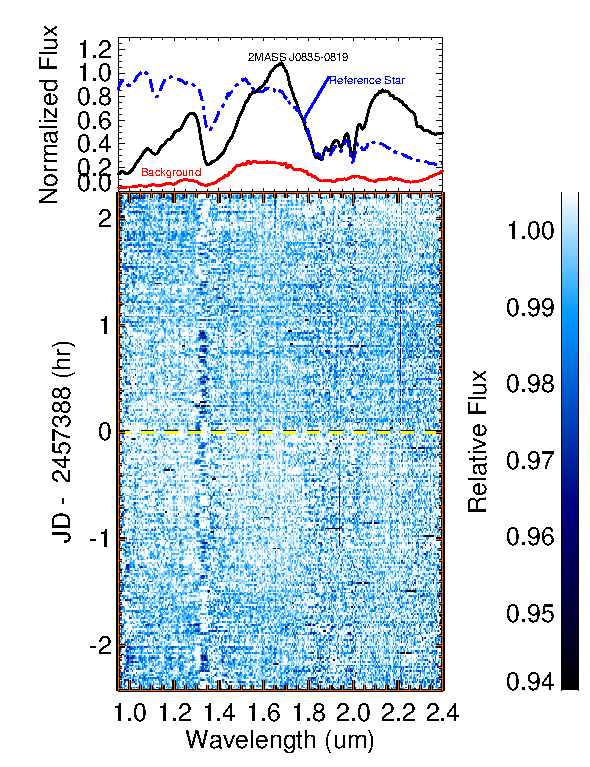
\includegraphics[width=0.5\textwidth]{specphot_j0835.pdf}
	\label{fig:specphot0835}
	}
\subfloat[2MASS J1821]{
	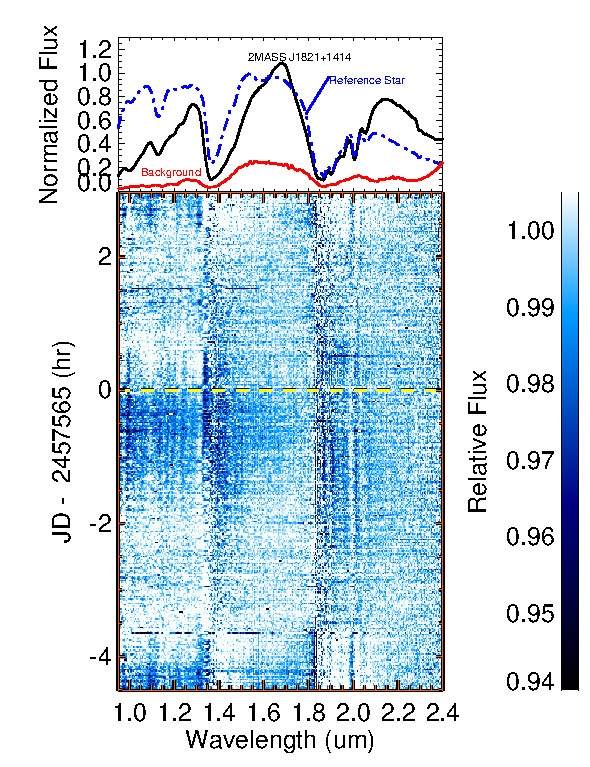
\includegraphics[width=0.5\textwidth]{specphot_j1821.pdf}
	\label{fig:specphot1821}
	}
	\caption{Top Panels: The target stars' median raw spectrum compared with the reference star. The areas near 1.4 and 1.8 $\mu$m are contaminated by telluric water absorption. The reference stars have significantly bluer spectra than the brown dwarfs. Bottom Panels: Dynamic spectra of each brown dwarf system.}
	\label{fig:specphot}
	\vspace{0.1in}
\end{figure*} 

Figure \ref{fig:specphot} shows the dynamic spectra for both brown dwarfs with the individual spectra of the target and reference stars on the upper panels.
At the $\lesssim 1$\% level, 2MASS J0835 shows no variations or systematics.
2MASS J1821 on the other hand, shows a periodic signal that is strongest at the short wavelength and gradually gets smaller toward longer wavelengths.
2MASS J1821 also exhibits systematic trends near strong slopes in the raw spectra due to telluric absorption bands.

\begin{figure*}[!t]
\centering
\subfloat[2MASS J0835]{
	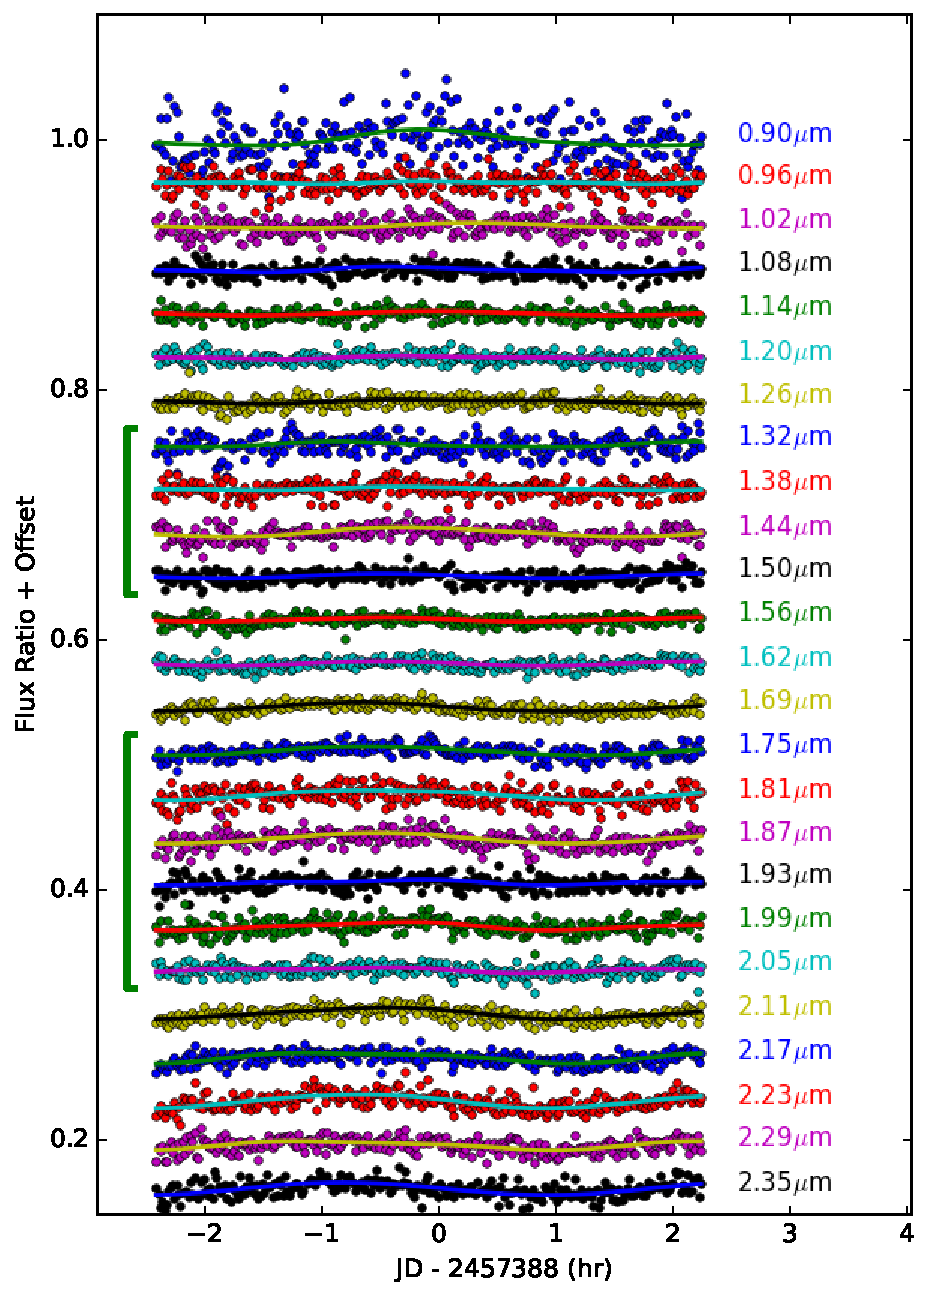
\includegraphics[width=0.5\textwidth]{2mass_0835_t_series.pdf}
	\label{fig:tserPhase0835}
	}
\subfloat[2MASS J1821]{
	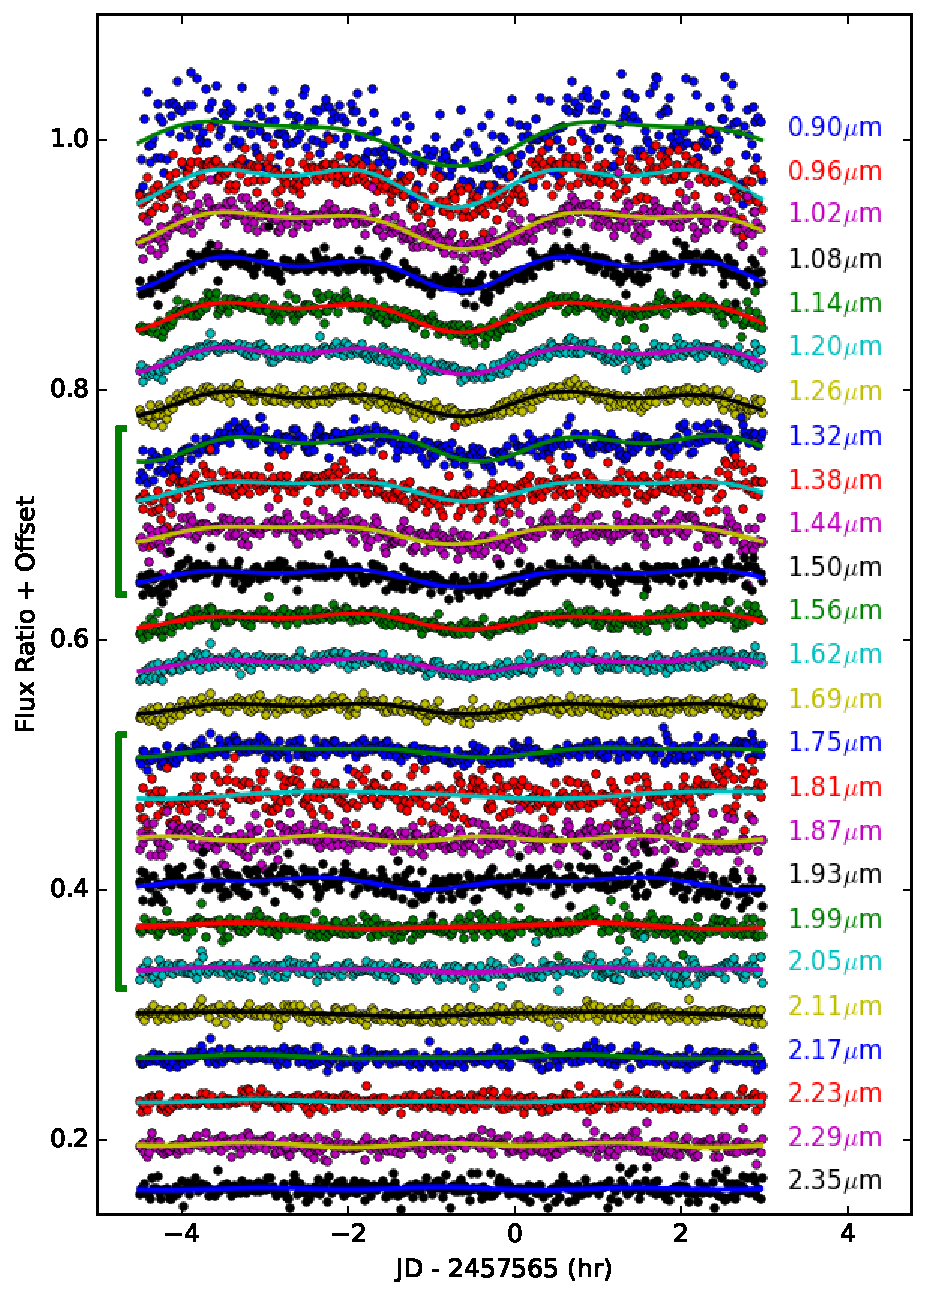
\includegraphics[width=0.5\textwidth]{2mass_1821_t_series.pdf}
	\label{fig:tserPhase1821}
	}
	\caption{Time series for each system. Alternating colors are used to distinguished the light curves with offsets.}
	\label{fig:tserPfold}
\end{figure*} 

2MASS J0835 exhibits no periodic behavior whereas 2MASS 1821 shows large varations when phasing the dynamic spectra at the known rotation periods of the two brown dwarfs, shown in Figure \ref{fig:tserPfold}.
For 2MASS 1821, the variations are mostly sinusoidal and repeat over multiple rotations of the brown dwarf - the exception is wavelengths near telluric features, such as 1.43~$\mu$m and 1.79~$\mu$m.


\section{Sinusoidal Model Fits}\label{sec:ModelFits}

We fit the time series of each brown dwarf in 25 spectral bins each to assess the wavelength-dependent nature of their variations.
The simple model can be described as 
\begin{equation}
F(t) = A * \sin(2 \pi (t - t_0)/\tau) + B t + C
\end{equation}
where $F$ is the flux as a function of time ($t$), A is the amplitude of the variations, $t_0$ is the time offset of the variations and $\tau$ is the and B and C are linear terms describing the baseline trend.
For the fits, we include a 4 free parameters: $A$, $t_0$, $B$ and $C$.
We fixed the sinusoidal period $\tau$ at the literature value of periodicity because there are also variations due to variable telluric variation that are not relevant to the brown dwarf system.
We imposed a prior that $A \geq 0$ so that a solution with a $\pi$ phase offset and negative amplitude isn't found.

\begin{figure*}[!]
\centering
\subfloat[2MASS J0835 - \colorbox{red}{fit might need more work} ]{
	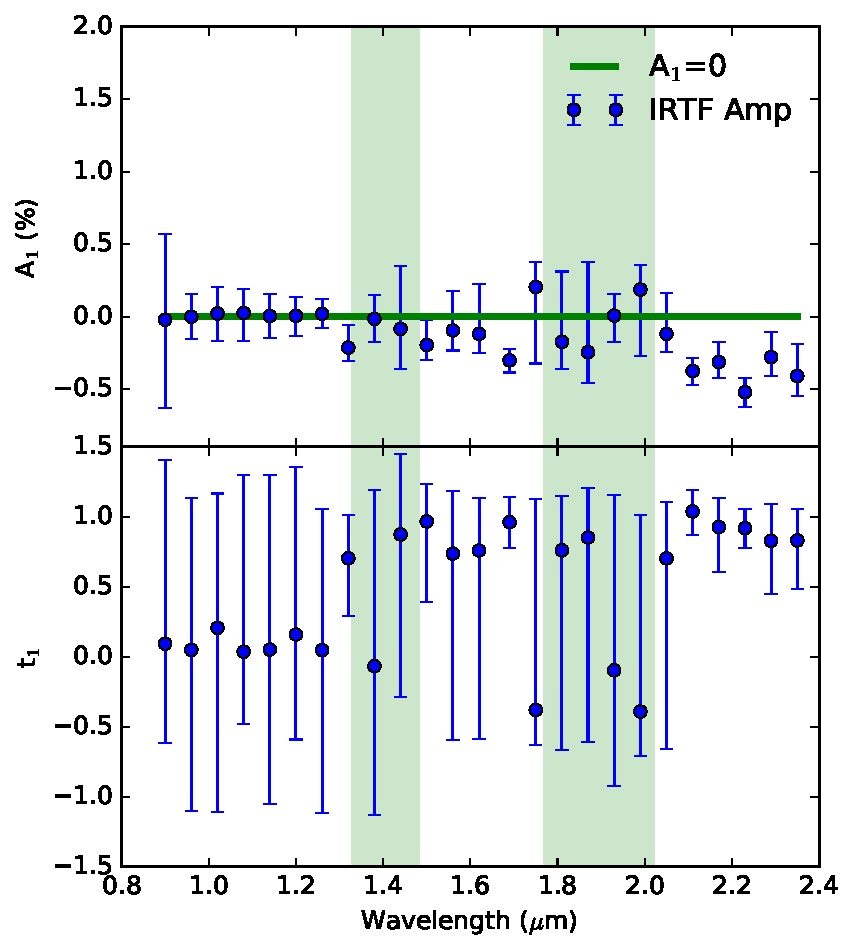
\includegraphics[width=0.5\textwidth]{amp_vs_wavl_j0835.pdf}
	\label{fig:ampspec0835}
	}
\subfloat[2MASS J1821]{
	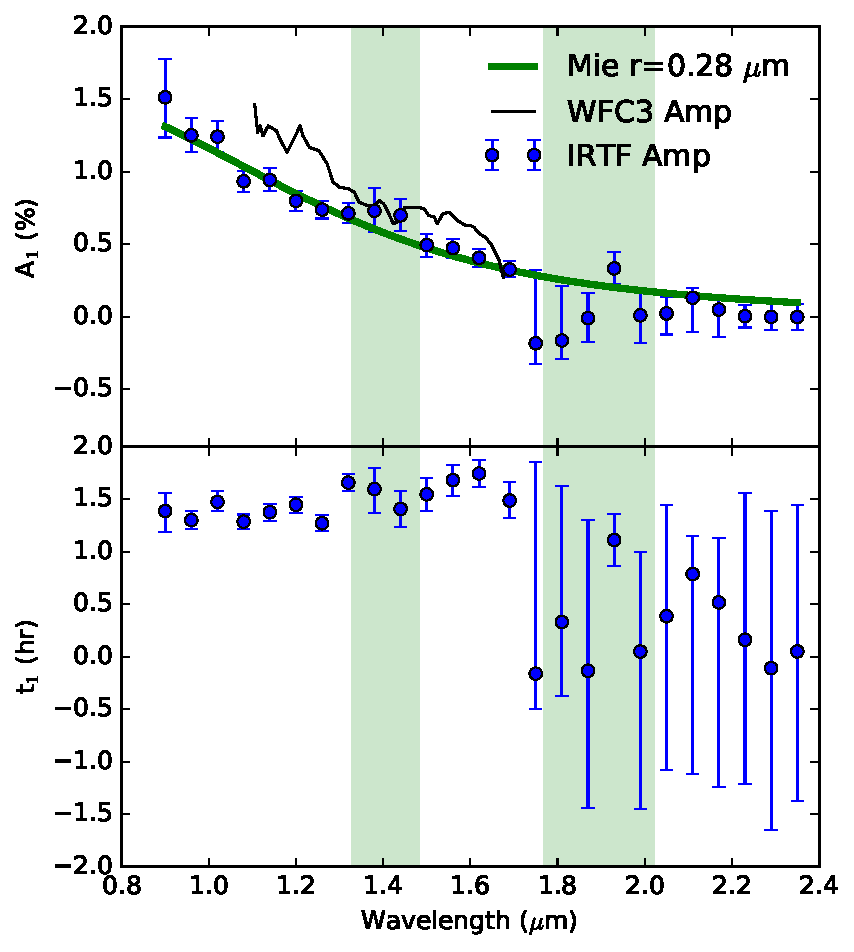
\includegraphics[width=0.5\textwidth]{amp_vs_wavl_j1821.pdf}
	\label{fig:ampspec1821}
	}
	\caption{Sine fit amplitude versus wavelength for each brown dwarf. The regions at 1.4~$\mu$m and 1.9~$\mu$m (shaded with a salmon color) are contaminated by telluric absorption so the variations can likely be due to telluric variability not corrected by the reference star.}
	\label{fig:ampSpec}
\end{figure*} 

Figure \ref{fig:ampSpec} shows the best fit amplitudes as a function of wavelength.
We use the standard deviation of points near minimum to estimate the noise in the flux time series.
The Levenberg-Marquardt chi-squared minimization code \texttt{mpfit} is used to fit each wavelength bin independently and propagate the errors in the flux time series to amplitude uncertainty.
The amplitude spectrum of 2MASS J0835 shown in Figure \ref{fig:ampspec0835} shows random fluctuations as a function of wavelength.
2MASS J1821, on the other hand, shows a clear decreasing trend as function of wavelength.
This was also observed in the shorter wavelength range of 1.1~$\mu$m to 1.7~$\mu$m in \citet{yang2016exStormsBD}.

This type of wavelength trend was also recently observed for WISEP J004701.06+680352.1 \citep{lew2016w0047}, which has a much $J-K$ 2.55 spectrum.
In WISEP J0047, the wavelength trend could be fit by $\sim 0.4~\mu$m forsterite grains.

%    \begin{figure}[!ht]
%    \centering
%    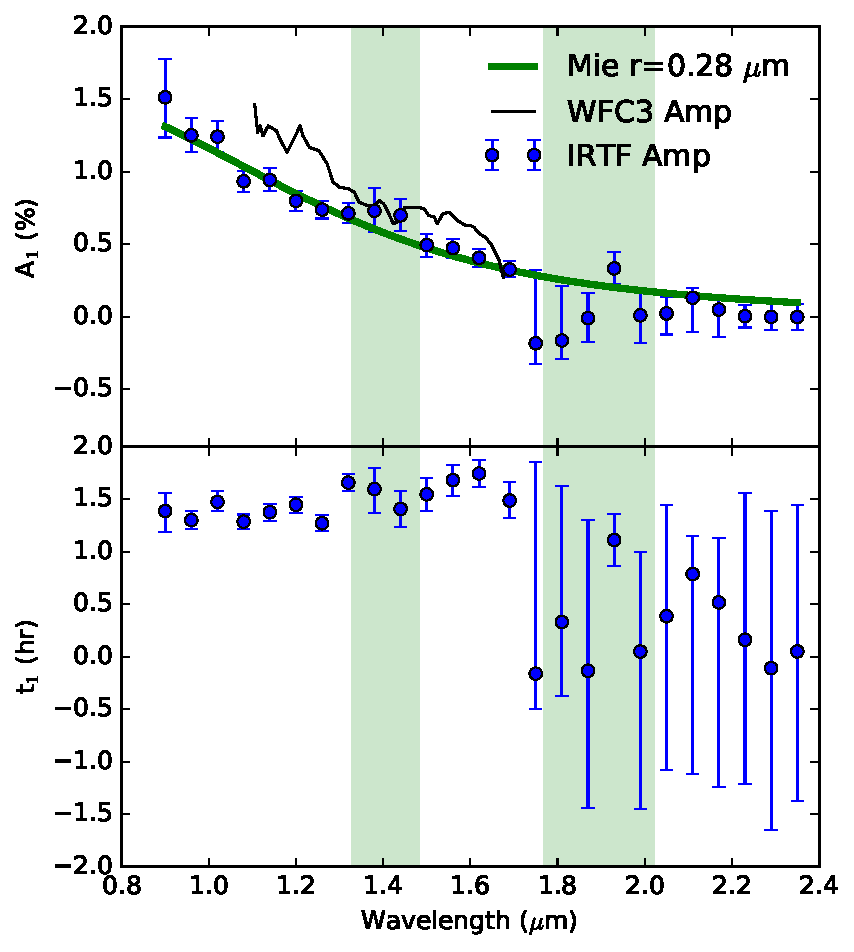
\includegraphics[width=0.5\textwidth]{amp_vs_wavl_j1821.pdf}
%    \caption{Sine fit amplitude versus wavelength for 2MASS J1821. The regions at 1.4~$\mu$m and 1.9~$\mu$m are contaminated by telluric absorption so the variations can likely be due to telluric variability not corrected by the reference star.}\label{fig:DHSRes}
%    \end{figure}

\subsection{Mie Scattering Fit}

We model the wavelength dependence of 2MASS 1821 as an optically thin cloud layer consisting of a log-normal distribution of particle sizes.
In this simple model, the amplitude of the variability is directly proportional to the opacity or $Q_{ext}$ of the particles.
We model the extinction coefficient, $Q_{ext}$ from the \texttt{IDL} Mie theory code \texttt{mie\_single.pro} \citep{grainger04} to calculate the extinction as a function of wavelength.
We use the complex indices of refraction from \citet{dorschner95pyrox} for Mg-rich pyroxene grains (MgSiO$_3$).
For the particle size distribution we assume a log-normal distribution around a characteristic size with a distribution $\sigma$ of 0.5.

\begin{figure}
\begin{centering}
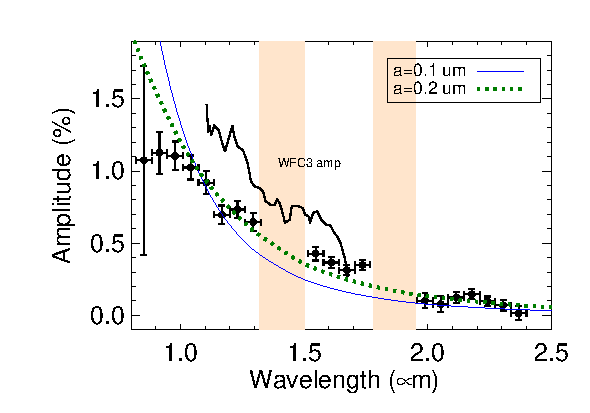
\includegraphics[width=0.5\textwidth]{amp_vs_wavl_j1821_mie_sc.pdf}
\caption{Sine fit amplitude versus wavelength excluding the wavelength regions contaminated by telluric absorption. with simple Mie scattering models with a log-normal particle size distribution centered at 0.1 and 0.2~$\mu$m. Also shown in the figure is the WFC3 amplitude from \citet{yang2015hstRotBD}. The WFC3 observations were from a different epoch, with different cloud coverage.}\label{fig:ampspec1821mie}
\end{centering}
\end{figure}

Figure \ref{fig:ampspec1821mie} shows the simple Mie scattering model as compared to the data for two example particle sizes of 0.1~$\mu$m and 0.2~$\mu$m.
In these cases the reduced chi-squared values are 9.6 and 2.5 respectively, when ignoring the points within the shaded telluric contamination regions.

\citet{yang2015hstRotBD} also observe wavelength-dependent variability of 2MASS J1821 with the Hubble Space Telescope's (HST's) Wide Field Camera (WFC3) over 2 visits of 3 orbits each.
Their maximum over minimum flux spectrum is converted to an amplitude spectrum by assuming that the amplitude is half the difference in maximum and minimum flux, which can be shown to be 
\begin{equation}
A  = \frac{f_R - 1}{f_R + 1}
\end{equation}\label{eq:ampFromRatio}
where $f_R$ is the flux ratio of the maximum over minimum flux.

The WFC3 amplitude spectrum is shown with the data in Figure \ref{fig:ampspec1821mie}.
There is a multiplicative offset between the IRTF and WFC3 spectrum because they were taken at different epochs and therefore different spatial cloud and temperature distributions.
The WFC3 spectrum is not affected by the telluric absorption the way the SpeX data is.
\citet{yang2015hstRotBD} find that the WFC3 spectrum has no significant water vapor absorption which indicates a high haze layer in 2MASS J1821, consistent with our Mie scattering fit.

\subsection{Spot Model Fit}

\begin{figure}
\begin{centering}
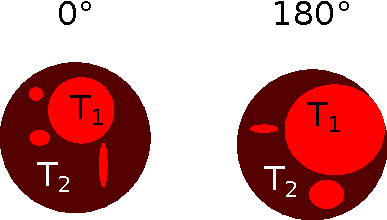
\includegraphics[width=0.4\textwidth]{temperature_drawing.pdf}
\caption{A simple two region model with two different temperatures and different areal fractions for longitudes 0\degree\ and 180\degree.}\label{fig:tdiffschem}
\end{centering}
\end{figure}

Another simple model we attempt is a spot model - that the brown dwarf spectral variability has to do with a non-uniform temperature distribution on the brown dwarf in the same way that starspots modulate the brightness of hydrogen burning stars as they spin.
In Figure \ref{fig:ampspec1821tdiff}, we fit the same amplitude spectrum as in Figure \ref{fig:ampspec1821mie}.
This time we model the data with two temperature regions as shown in Figure \ref{fig:tdiffschem} with two opposite longitudes of the planet at the brightness minimum and maximum.
We assume that are each in local thermodynamic equilibrium (LTE) so that the flux is proportional to the Planck function times the areal coverage.
The flux ratio between maximum and minimum flux is then
\begin{equation}
f_{R,\lambda} = \frac{\alpha_1 B_\lambda(T_1) + (1-\alpha_1) B_\lambda(T_2)}{\alpha_2 B_\lambda(T_1) + (1-\alpha_2) B_\lambda(T_2)}
\end{equation}
where $\alpha_1$ and $\alpha_2$ are the areal fractions of the two temperature layers limited to [0,1], $B_\lambda$ is the Planck function, and $T_1$ and $T_2$ are the temperatures of the two levels.
Using equation \ref{eq:ampFromRatio}, the amplitude then becomes
\begin{equation}
A_\lambda = \frac{\left(\alpha_1 - \alpha_2 \right) \left(B_\lambda(T_1) - B_\lambda(T_2) \right)}{\left(\alpha_1 + \alpha_2\right) B_\lambda(T_1) + \left(2 - \alpha_1 - \alpha_2\right) B_\lambda(T_2)}.
\end{equation}
If the temperature difference is significant so that one Planck function is in the Wien's limit while the other is in the Rayleigh Jeans tail, the cooler temperature essentially becomes black and the contrast approaches a constant for short wavelengths.
If we ignore projection effects for small area coverage, the effective temperature is 
\begin{equation}
\sigma T_{eff}^4 \approx (\alpha_1 + \alpha_2) \sigma T_1^4 + (2 - \alpha_1 - \alpha_2) \sigma T_2^4
\end{equation}
where $\sigma$ is the Stephan-Boltzmann constant.

Our model best-fits the data with $\alpha_i << $1 and also with much lower temperatures than equilibrium, shown in Figure \ref{fig:ampspec1821tdiff}.
This model has a reduced chi-squared of 1.3, consistent with the data, but not with the effective temperature.
If we restrict the model to be a two-faced model where $\alpha_1$ = 1 and $\alpha_2$ = 0, so that the two halves of the brown dwarf are different temperatures, the best-fit is a poor match to the data, also shown in Figure \ref{fig:ampspec1821tdiff} with a $\bar{\chi}^2$ = 15.
Finally, we attempt a model where we restrict the temperature limits to [1300,2500] to ensure that the final effective temperature is close to the measured 1600 K \citep{gagne2015banyan7}.
The best fit model has $T_{eff} \approx $1590 K, but pushes to the edges of our prior with $T_1$ = 2500 K and $T_2$ = 1300 K.
The temperature contrasts in these models (with the exception of the two-faced model which poorly matches the data) are significantly more than the expected 50 K horizontal temperature variations expected in circulation models \citep{showman2013bdgpDynamics}.
Therefore, we suspect that hot or cold spots on the surface a are a less likely scenario to explain the variability of 2MASS 1821.

\begin{figure}
\begin{centering}
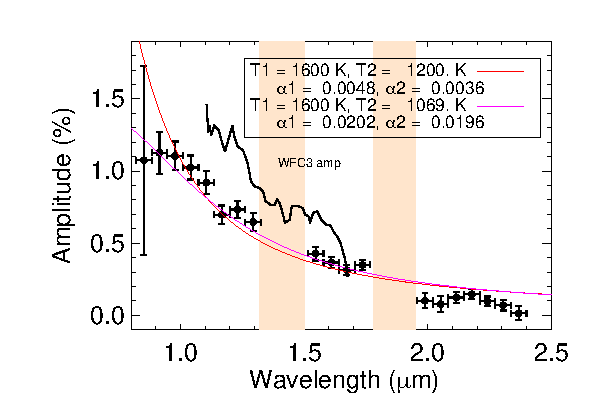
\includegraphics[width=0.5\textwidth]{amp_vs_wavl_j1821_t_diff.pdf}
\caption{The same data as in Figure \ref{fig:ampspec1821mie}. We fit the data with a two region model that assumes the effective temperature of the brown dwarf and a cooler temperature.}\label{fig:ampspec1821tdiff}
\end{centering}
\end{figure}
% Command used:
% plot_rad_vs_wavl,/amp,/shadetell,custxrange=[0.8,2.5],custyrange=[-0.1,1.9],/showYang,/twoTreg





\section{Conclusions}\label{sec:conclusions}

We observed two brown dwarfs of spectral type L4-L5: 2MASS 1821 and 2MASS 0835.
These brown dwarfs have temperatures near the condensation temperatures of MgSiO$_3$ and Mg$_2$SiO$_4$.
We obtained high precision ground-based spectrophotometry of both systems to measure the variability spectra of these systems with the IRTF.
After fitting sinusoids to both of the time series, we find that 2MASS 0835 has low levels of variability and not wavelength dependence.

2MASS J1821 shows significant variability up to the 1.1\% amplitude at short wavelengths (0.8$\mu$m) which decreases towards the near infrared (2.4$\mu$m).
This is consistent with HST measurements for the system that show a gradual decrease in variability amplitude with wavelength \citep{yang2016exStormsBD} from 1.1$\mu$m to 1.7 $\mu$m with no decrease in the water vapor band.
The lack of the water vapor band gives evidence of a high altitude aerosol layer in the atmosphere.

We fit the variability amplitude spectrum with an optically thin Mie scattering model and find it is consistent with Mg-rich pyroxene grains with sub-micron sized particles.
A log-normal particle size distribution with a median of 0.2$\mu$m fits the data with a $\bar{\chi^2}$ of 2.5.
We also model the wavelength dependence with a spotted surface model with two different Planck functions covering different spatial regions.
The two temperature region model can fit variability amplitude spectrum well within errors, but gives implausible temperatures and temperature differences.
Therefore, we favor the Mie scattering model as a better explanation for the variability amplitude spectrum.

\section{Acknowledgements}
Thanks to Vivien Parmentier for useful discussions on cloud versus a spotted temperature model.
Funding for the E Schlawin is provided by NASA Goddard Spaceflight Center.
This research has made use of the Exoplanet Orbit Database and the Exoplanet Data Explorer at exoplanets.org.
This research made use of the \texttt{astropy} package \citep{astropy2013}.

\appendix

\section{Color-Magnitude Diagram}
\begin{figure}
\begin{centering}
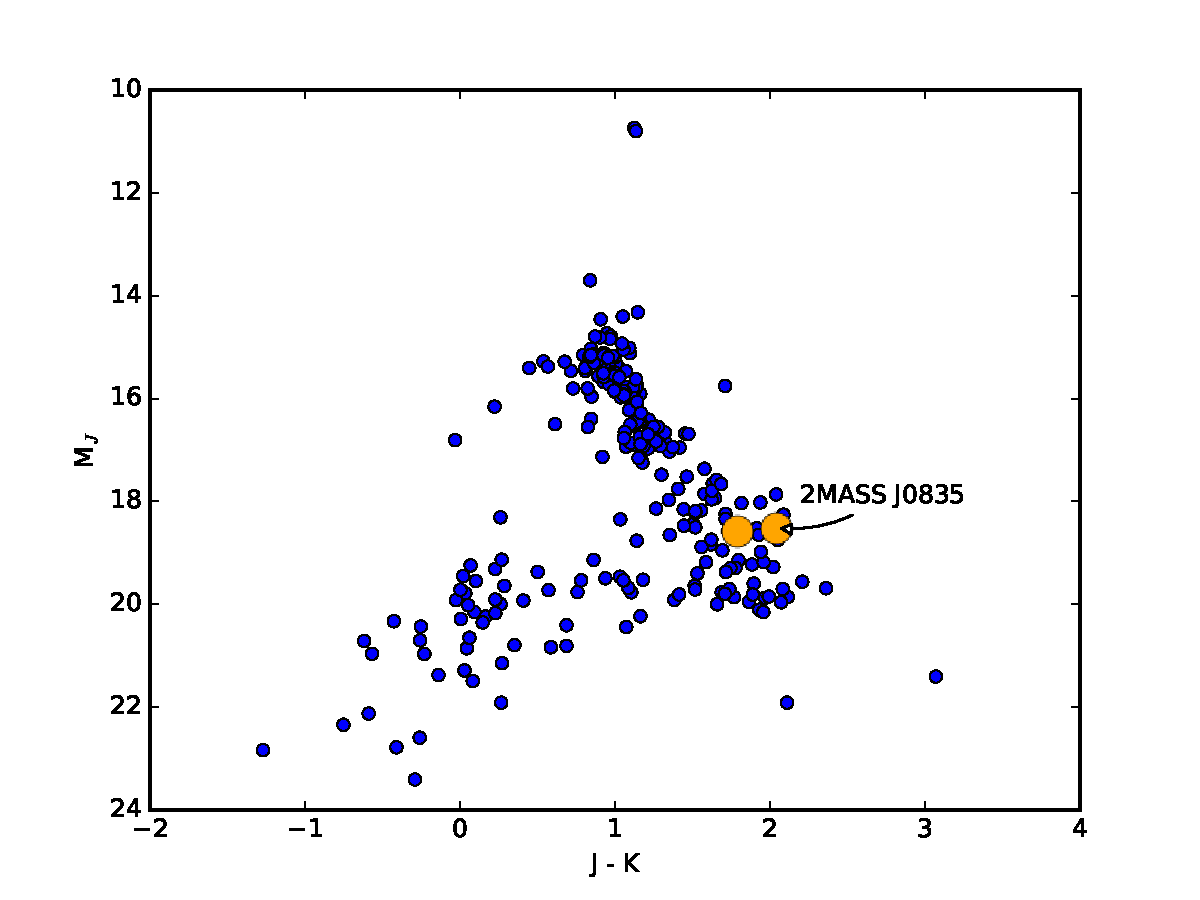
\includegraphics[width=0.5\textwidth]{color_mag.pdf}
\caption{Color-Magnitude diagram from \citet{dupuy2012ltparallax}.}\label{fig:CMD}
\end{centering}
\end{figure}

%If  used, this work made use of the \texttt{astropy} package \citep{astropy2013}.
%If used, some data was collected from the Open Exoplanet Catalogue \citep{rein2012openExoCat}.

%% In a manner similar to \objectname authors can provide links to dataset
%% hosted at participating data centers via the \dataset{} command.  The
%% second curly bracket argument is printed in the text while the first
%% parentheses argument serves as the valid data set identifier.  Large
%% lists of data set are best provided in a table (see Table 3 for an example).
%% Valid data set identifiers should be obtained from the data center that
%% is currently hosting the data.
%%
%% Note that AASTeX interprets everything between the curly braces in the 
%% macro as regular text, so any special characters, e.g. "#" or "_," must be 
%% preceded by a backslash. Otherwise, you will get a LaTeX error when you 
%% compile your manuscript.  Special characters do not 
%% need to be escaped in the optional, square-bracket argument.



%% In this section, we use  the \subsection command to set off
%% a subsection.  \footnote is used to insert a footnote to the text.

%% Observe the use of the LaTeX \label
%% command after the \subsection to give a symbolic KEY to the
%% subsection for cross-referencing in a \ref command.
%% You can use LaTeX's \ref and \label commands to keep track of
%% cross-references to sections, equations, tables, and figures.
%% That way, if you change the order of any elements, LaTeX will
%% automatically renumber them.

%% This section also includes several of the displayed math environments
%% mentioned in the Author Guide.


%% The equation environment wil produce a numbered display equation.


%% The \notetoeditor{TEXT} command allows the author to communicate
%% information to the copy editor.  This information will appear as a
%% footnote on the printed copy for the manuscript style file.  Nothing will
%% appear on the printed copy if the preprint or
%% preprint2 style files are used.

%% The eqnarray environment produces multi-line display math. The end of
%% each line is marked with a \\. Lines will be numbered unless the \\
%% is preceded by a \nonumber command.
%% Alignment points are marked by ampersands (&). There should be two
%% ampersands (&) per line.

%% Putting eqnarrays or equations inside the mathletters environment groups
%% the enclosed equations by letter. For instance, the eqnarray below, instead
%% of being numbered, say, (4) and (5), would be numbered (4a) and (4b).
%% LaTeX the paper and look at the output to see the results.

%% This section contains more display math examples, including unnumbered
%% equations (displaymath environment). The last paragraph includes some
%% examples of in-line math featuring a couple of the AASTeX symbol macros.

%% The displaymath environment will produce the same sort of equation as
%% the equation environment, except that the equation will not be numbered
%% by LaTeX.
%% If you wish to include an acknowledgments section in your paper,
%% separate it off from the body of the text using the \acknowledgments
%% command.

%% Included in this acknowledgments section are examples of the
%% AASTeX hypertext markup commands. Use \url without the optional [HREF]
%% argument when you want to print the url directly in the text. Otherwise,
%% use either \url or \anchor, with the HREF as the first argument and the
%% text to be printed in the second.

\acknowledgments



%% To help institutions obtain information on the effectiveness of their
%% telescopes, the AAS Journals has created a group of keywords for telescope
%% facilities. A common set of keywords will make these types of searches
%% significantly easier and more accurate. In addition, they will also be
%% useful in linking papers together which utilize the same telescopes
%% within the framework of the National Virtual Observatory.
%% See the AASTeX Web site at http://aastex.aas.org/
%% for information on obtaining the facility keywords.

%% After the acknowledgments section, use the following syntax and the
%% \facility{} macro to list the keywords of facilities used in the research
%% for the paper.  Each keyword will be checked against the master list during
%% copy editing.  Individual instruments or configurations can be provided 
%% in parentheses, after the keyword, but they will not be verified.

%{\it Facilities:} \facility{Nickel}, \facility{HST (STIS)}, \facility{CXO (ASIS)}.

%% Appendix material should be preceded with a single \appendix command.
%% There should be a \section command for each appendix. Mark appendix
%% subsections with the same markup you use in the main body of the paper.

%% Each Appendix (indicated with \section) will be lettered A, B, C, etc.
%% The equation counter will reset when it encounters the \appendix
%% command and will number appendix equations (A1), (A2), etc.

\appendix


%% The reference list follows the main body and any appendices.
%% Use LaTeX's thebibliography environment to mark up your reference list.
%% Note \begin{thebibliography} is followed by an empty set of
%% curly braces.  If you forget this, LaTeX will generate the error
%% "Perhaps a missing \item?".
%%
%% thebibliography produces citations in the text using \bibitem-\cite
%% cross-referencing. Each reference is preceded by a
%% \bibitem command that defines in curly braces the KEY that corresponds
%% to the KEY in the \cite commands (see the first section above).
%% Make sure that you provide a unique KEY for every \bibitem or else the
%% paper will not LaTeX. The square brackets should contain
%% the citation text that LaTeX will insert in
%% place of the \cite commands.

%% We have used macros to produce journal name abbreviations.
%% AASTeX provides a number of these for the more frequently-cited journals.
%% See the Author Guide for a list of them.

%% Note that the style of the \bibitem labels (in []) is slightly
%% different from previous examples.  The natbib system solves a host
%% of citation expression problems, but it is necessary to clearly
%% delimit the year from the author name used in the citation.
%% See the natbib documentation for more details and options.

\bibliographystyle{apj}
\bibliography{bd_biblio}

%\clearpage

%% Use the figure environment and \plotone or \plottwo to include
%% figures and captions in your electronic submission.
%% To embed the sample graphics in
%% the file, uncomment the \plotone, \plottwo, and
%% \includegraphics commands
%%
%% If you need a layout that cannot be achieved with \plotone or
%% \plottwo, you can invoke the graphicx package directly with the
%% \includegraphics command or use \plotfiddle. For more information,
%% please see the tutorial on "Using Electronic Art with AASTeX" in the
%% documentation section at the AASTeX Web site, http://aastex.aas.org/
%%
%% The examples below also include sample markup for submission of
%% supplemental electronic materials. As always, be sure to check
%% the instructions to authors for the journal you are submitting to
%% for specific submissions guidelines as they vary from
%% journal to journal.

%% This example uses \plotone to include an EPS file scaled to
%% 80% of its natural size with \epsscale. Its caption
%% has been written to indicate that additional figure parts will be
%% available in the electronic journal.

%\begin{figure}
%\epsscale{.80}
%\plotone{f1.eps}
%\caption{Derived spectra for 3C138 \citep[see][]{heiles03}. Plots for all sources are available
%in the electronic edition of {\it The Astrophysical Journal}.\label{fig1}}
%\end{figure}

%\clearpage

%% Here we use \plottwo to present two versions of the same figure,
%% one in black and white for print the other in RGB color
%% for online presentation. Note that the caption indicates
%% that a color version of the figure will be available online.
%%

%\begin{figure}
%\plottwo{f2.eps}{f2_color.eps}
%\caption{A panel taken from Figure 2 of \citet{rudnick03}. 
%See the electronic edition of the Journal for a color version 
%of this figure.\label{fig2}}
%\end{figure}

%% This figure uses \includegraphics to scale and rotate the still frame
%% for an mpeg animation.

%\begin{figure}
%\includegraphics[angle=90,scale=.50]{f3.eps}
%\caption{Animation still frame taken from \citet{kim03}.
%This figure is also available as an mpeg
%animation in the electronic edition of the
%{\it Astrophysical Journal}.}
%\end{figure}

%% If you are not including electonic art with your submission, you may
%% mark up your captions using the \figcaption command. See the
%% User Guide for details.
%%
%% No more than seven \figcaption commands are allowed per page,
%% so if you have more than seven captions, insert a \clearpage
%% after every seventh one.

%% Tables should be submitted one per page, so put a \clearpage before
%% each one.

%% Two options are available to the author for producing tables:  the
%% deluxetable environment provided by the AASTeX package or the LaTeX
%% table environment.  Use of deluxetable is preferred.
%%

%% Three table samples follow, two marked up in the deluxetable environment,
%% one marked up as a LaTeX table.

%% In this first example, note that the \tabletypesize{}
%% command has been used to reduce the font size of the table.
%% We also use the \rotate command to rotate the table to
%% landscape orientation since it is very wide even at the
%% reduced font size.
%%
%% Note also that the \label command needs to be placed
%% inside the \tablecaption.

%% This table also includes a table comment indicating that the full
%% version will be available in machine-readable format in the electronic
%% edition.

%% If you use the table environment, please indicate horizontal rules using
%% \tableline, not \hline.
%% Do not put multiple tabular environments within a single table.
%% The optional \label should appear inside the \caption command.



%% If the table is more than one page long, the width of the table can vary
%% from page to page when the default \tablewidth is used, as below.  The
%% individual table widths for each page will be written to the log file; a
%% maximum tablewidth for the table can be computed from these values.
%% The \tablewidth argument can then be reset and the file reprocessed, so
%% that the table is of uniform width throughout. Try getting the widths
%% from the log file and changing the \tablewidth parameter to see how
%% adjusting this value affects table formatting.

%% The \dataset{} macro has also been applied to a few of the objects to
%% show how many observations can be tagged in a table.


%% Tables may also be prepared as separate files. See the accompanying
%% sample file table.tex for an example of an external table file.
%% To include an external file in your main document, use the \input
%% command. Uncomment the line below to include table.tex in this
%% sample file. (Note that you will need to comment out the \documentclass,
%% \begin{document}, and \end{document} commands from table.tex if you want
%% to include it in this document.)

%% \input{table}

%% The following command ends your manuscript. LaTeX will ignore any text
%% that appears after it.

\end{document}

%%
%% End of file `sample.tex'.
